\chapter{Design}

The HaptiQ aims to solve some of the problems identifies in the related work. The hardware was developed using an iterative explorative process. Therefore the design phases largely overlap with the implementation ones. The API provided has also undergone through many iterations. In this chapter I will first discuss the earliest prototypes. Then the 4-HaptiQ and the 8-HaptiQ hardware designs are illustrated. Finally, a detailed overview of the API is provided.

\section{The Hardware}
\subsection{Early Prototypes}
The hardware design of the HaptiQ has been initially based on the HTP design. Similarly to the HTP, the HaptiQ also uses mini-servos to control its actuators. However, while the HTP controls only one actuator, the HaptiQ controls four or eight of them. It immediately follows that as the number of actuators increases, so do the number of servos and the size of the device. In order to minimise the size I designed three main prototypes by sketches (see Figure ~\ref{fig:HaptiQ-early-prototypes}). 

The first prototype extends the rotational axis in the xy plane (see Figure ~\ref{fig:first prototype}). The extension is designed as a gear that allows to choose combinations of three aligned actuators. An additional actuator would then be used to raise the selected actuators. This design reduces the number of servos, but all raised actuators will have the same height. Note that the focus of this design sketch was to minimise the number of servos, that is why actuators are shown as points, similar to Braille displays.

\begin{figure}
        \centering
        \begin{subfigure}[H]{0.5\textwidth}
                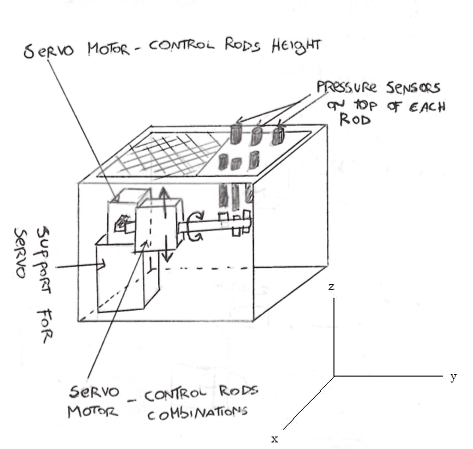
\includegraphics[width=\textwidth,height=\textwidth]{prototype1.png}
                \caption{Grid based}
                \label{fig:first prototype}
        \end{subfigure}%
        ~ %add desired spacing between images, e. g. ~, \quad, \qquad etc.
          %(or a blank line to force the subfigure onto a new line)
        \begin{subfigure}[H]{0.5\textwidth}
                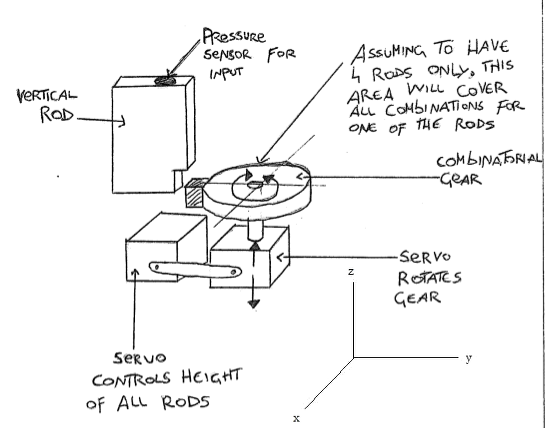
\includegraphics[width=\textwidth,height=\textwidth]{prototype2.png}
                \caption{Gear based}
                \label{fig:second prototype}
        \end{subfigure}
        ~ %add desired spacing between images, e. g. ~, \quad, \qquad etc.
          %(or a blank line to force the subfigure onto a new line)
        \begin{subfigure}[H]{0.5\textwidth}
                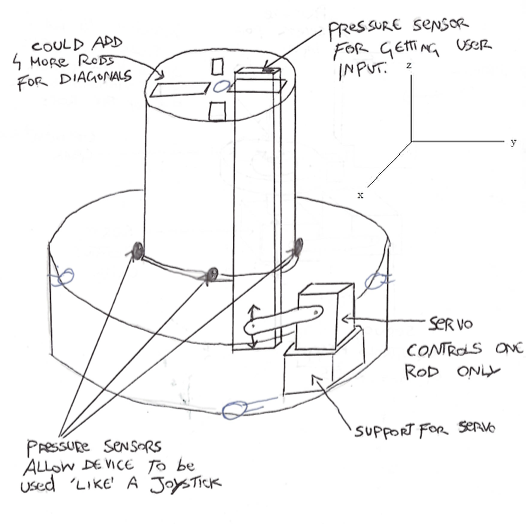
\includegraphics[width=\textwidth,height=\textwidth]{prototype3.png}
                \caption{One servo per actuator}
                \label{fig:third prototype}
        \end{subfigure}
        \caption{HaptiQ early prototypes}\label{fig:HaptiQ-early-prototypes}
\end{figure}

In the second prototype I tried to minimize the total number of servos to two. One servo would be used to rotate a combinatorial gear about the z-axis(see Figure ~\ref{fig:second prototype}). A second servo can then be used to raise the first servo with the gear it controls and all the rods. This approach can be consired very versatile and could allow an high number of actuators by keeping the number of servos always to two. Nonetheless, the actuators would all be at the same heights when raised as in the first prototype. Since height can be used to convey additional information, this prototype was discarded and a third prototype was created.

The third prototype does not focus on minimising the number of servos anymore, but rather on the possible functionalities that could be added to the HaptiQ. In this design each servo controls an actuator only and these are disposed circularly around the center of the device (see Figure ~\ref{fig:third prototype}). The device would have a "joystick" shape. Three pressure sensors could be added either at the bottom of the device or in between the internal and the external annuli. Using simple triangulation on the pressure sensors values, it could be possible to use the device like a gaming joystick and eventually augment its area of interaction. However, in one of the meetings with Saad, we realised that blind people would find this feature disrupting because understanding how far in the xy plane the device is augmented can become a challenging task. 

\subsection{4-HaptiQ}
The 4-HaptiQ is the first functional HaptiQ. This is an experimental project, with future work discussed in chapter 9, so I will occasionally refer to the device with the term prototype. This version has four actuators as shown in figure ~\ref{fig:HaptiQ reference static actuators}. Unlike the third of the early prototypes, the main focus is on the mechanics and functionalities aspects.
The most successful aspect of the HTP, most probably, is the use of a small servo to mechanically move the rod along the z-axis. Nonetheless, the mechanic design used in the HTP has some flows that the HaptiQ tries to solve. The HTP, in fact, transforms the rotational motion of the servo to a linear motion only by ensuring that the servo works under a small range and that the rod slices outside the device through a small opening.
In the HaptiQ the actuators slide through a guide that allows motion only in the z-direction. In addition, each servo is linked to its actuator by using one or more screws inserted in between small openings in the actuator (see Figures ~\ref{fig:HaptiQ MinPos} and ~\ref{fig:HaptiQ MaxPos}). 

\begin{figure}
        \centering
        \begin{subfigure}[H]{0.3\textwidth}
                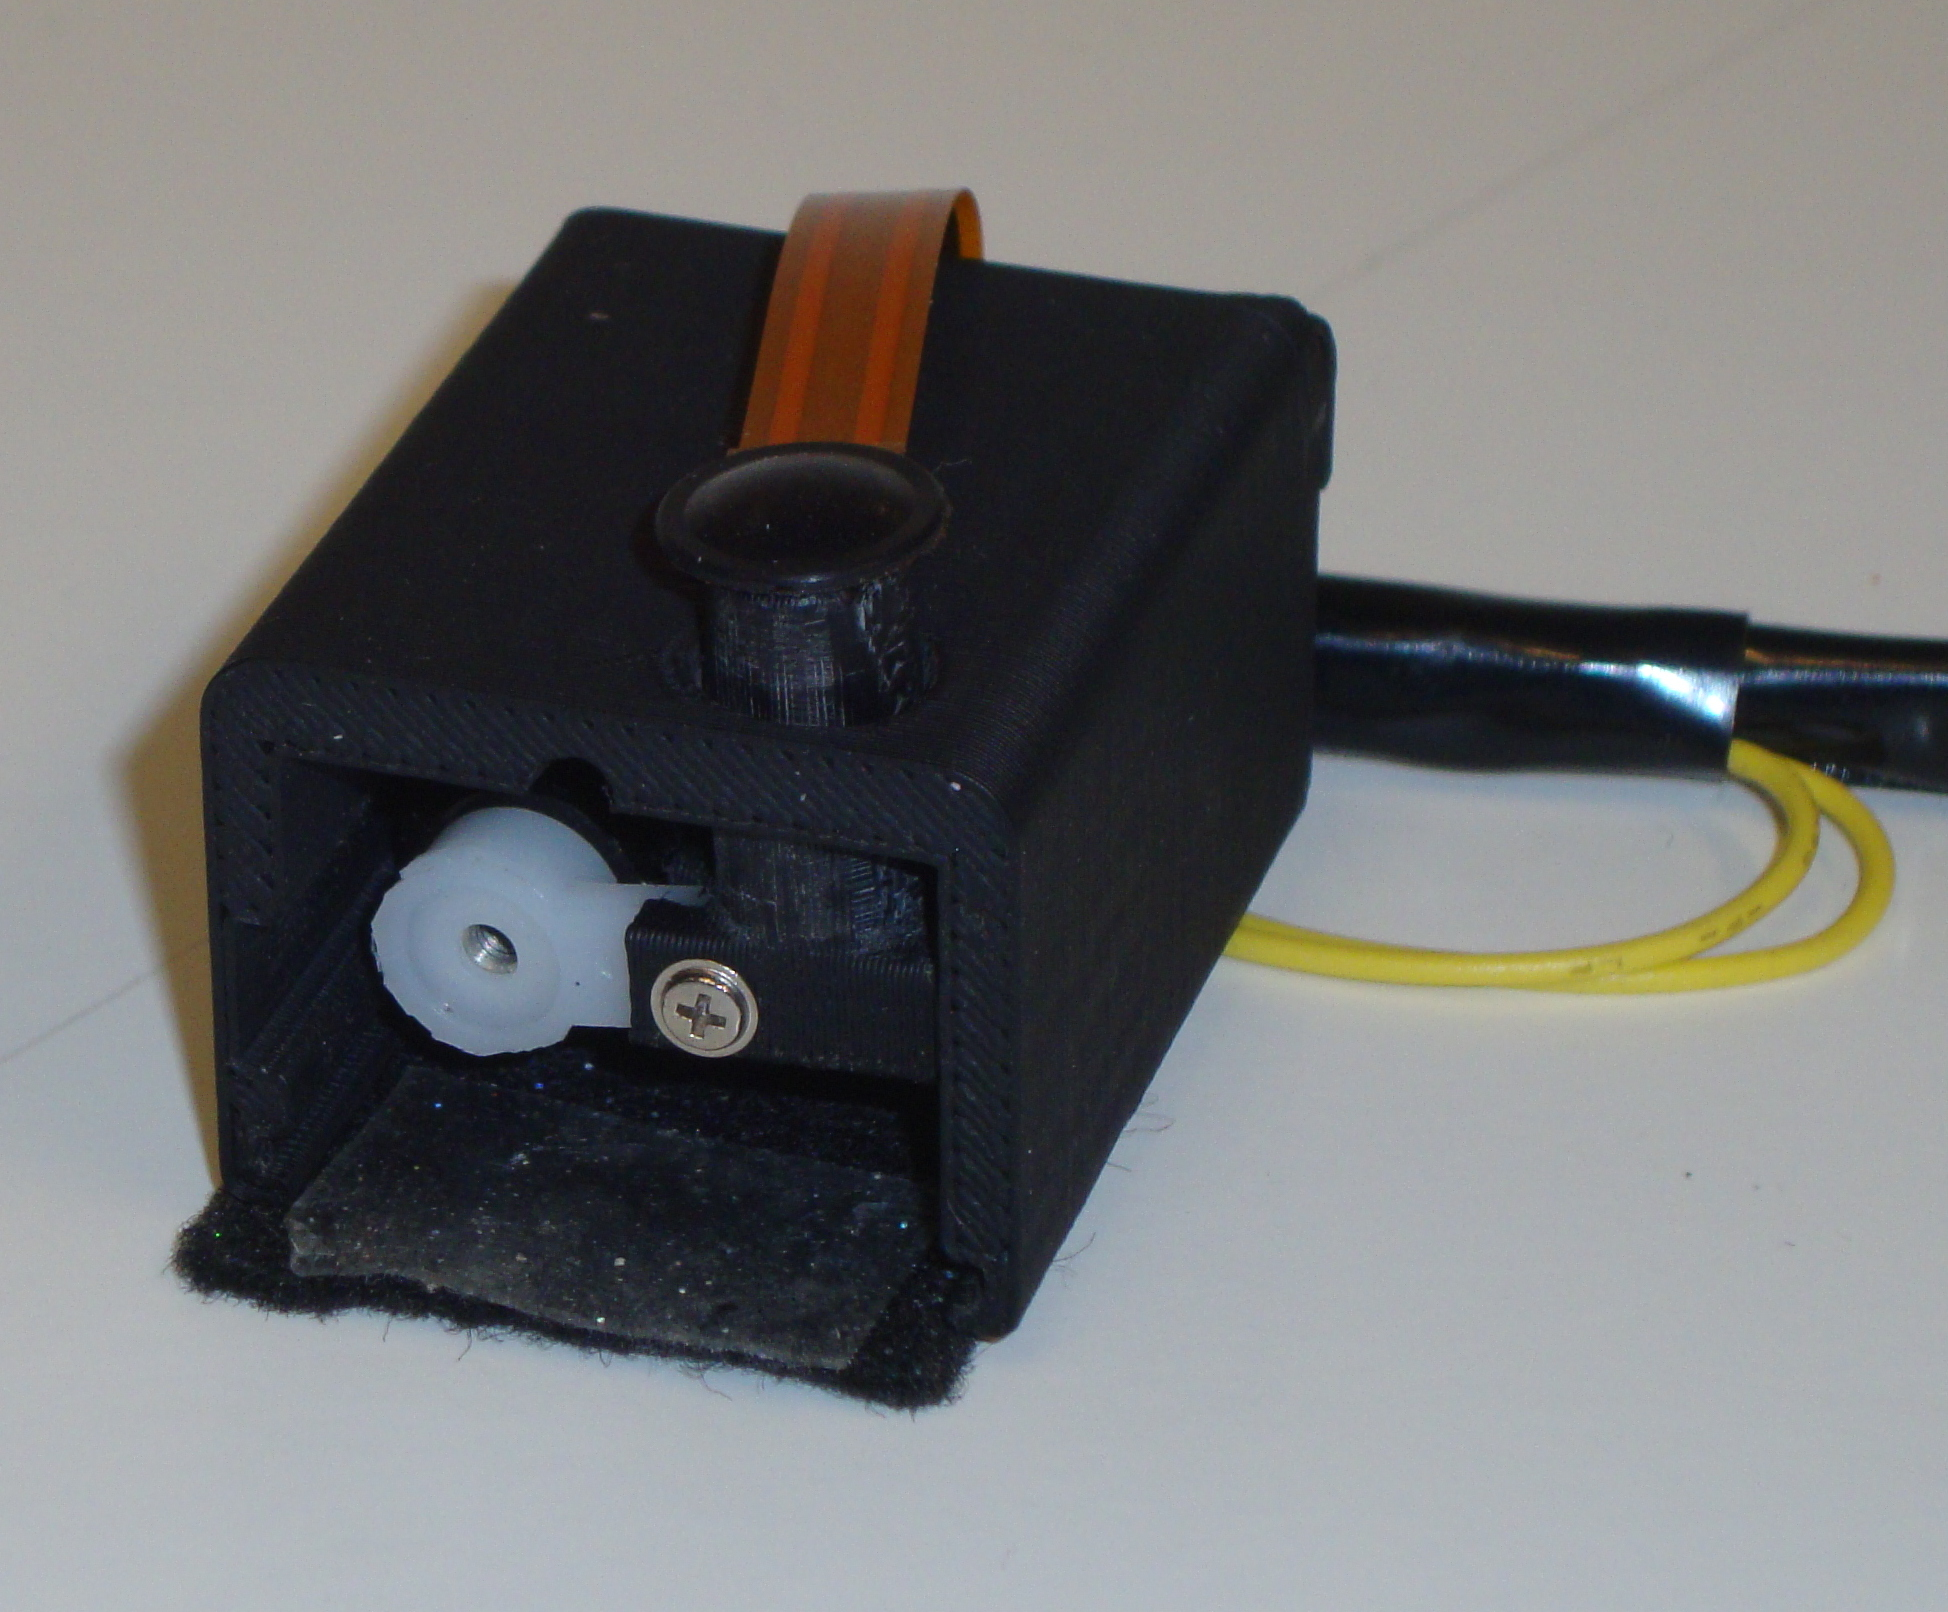
\includegraphics[width=\textwidth,height=\textwidth]{htp2.JPG}
                \caption{HTP}
                \label{fig:Mechanics HTP}
        \end{subfigure}%
        ~ %add desired spacing between images, e. g. ~, \quad, \qquad etc.
          %(or a blank line to force the subfigure onto a new line)
        \begin{subfigure}[H]{0.3\textwidth}
                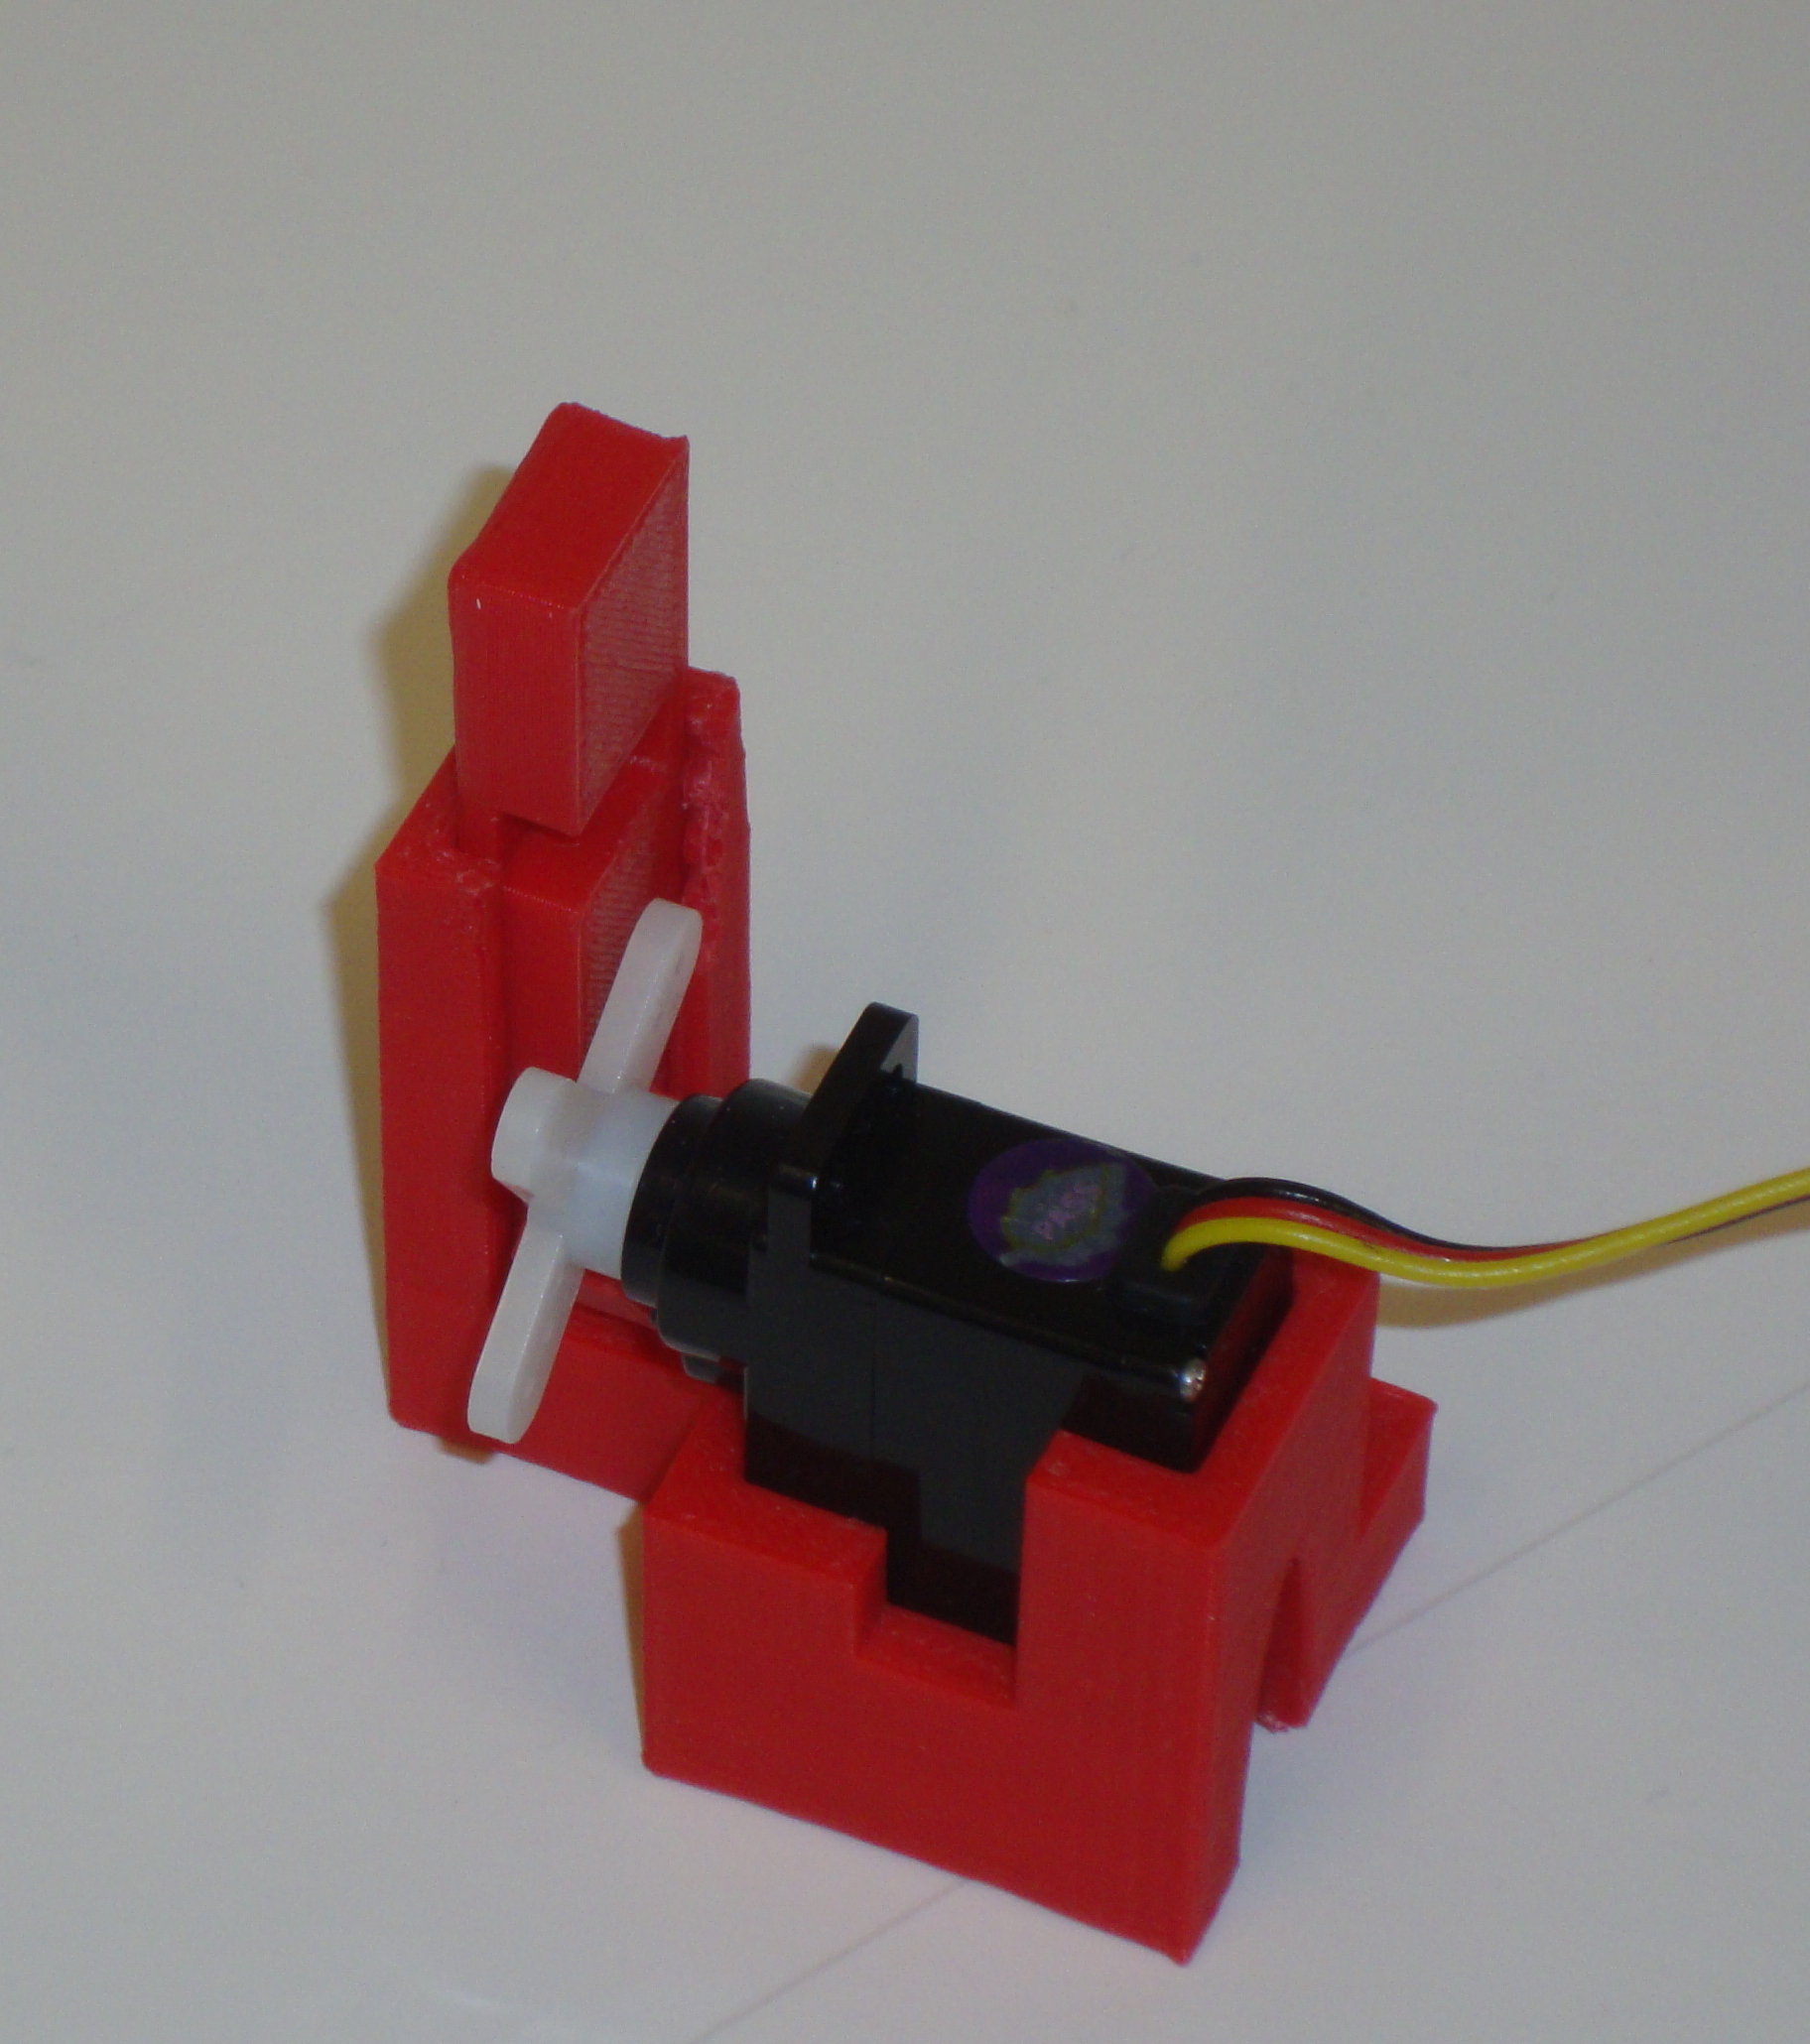
\includegraphics[width=\textwidth,height=\textwidth]{pos1.JPG}
                \caption{HaptiQ MinPos}
                \label{fig:HaptiQ MinPos}
        \end{subfigure}
        ~ %add desired spacing between images, e. g. ~, \quad, \qquad etc.
          %(or a blank line to force the subfigure onto a new line)
        \begin{subfigure}[H]{0.3\textwidth}
                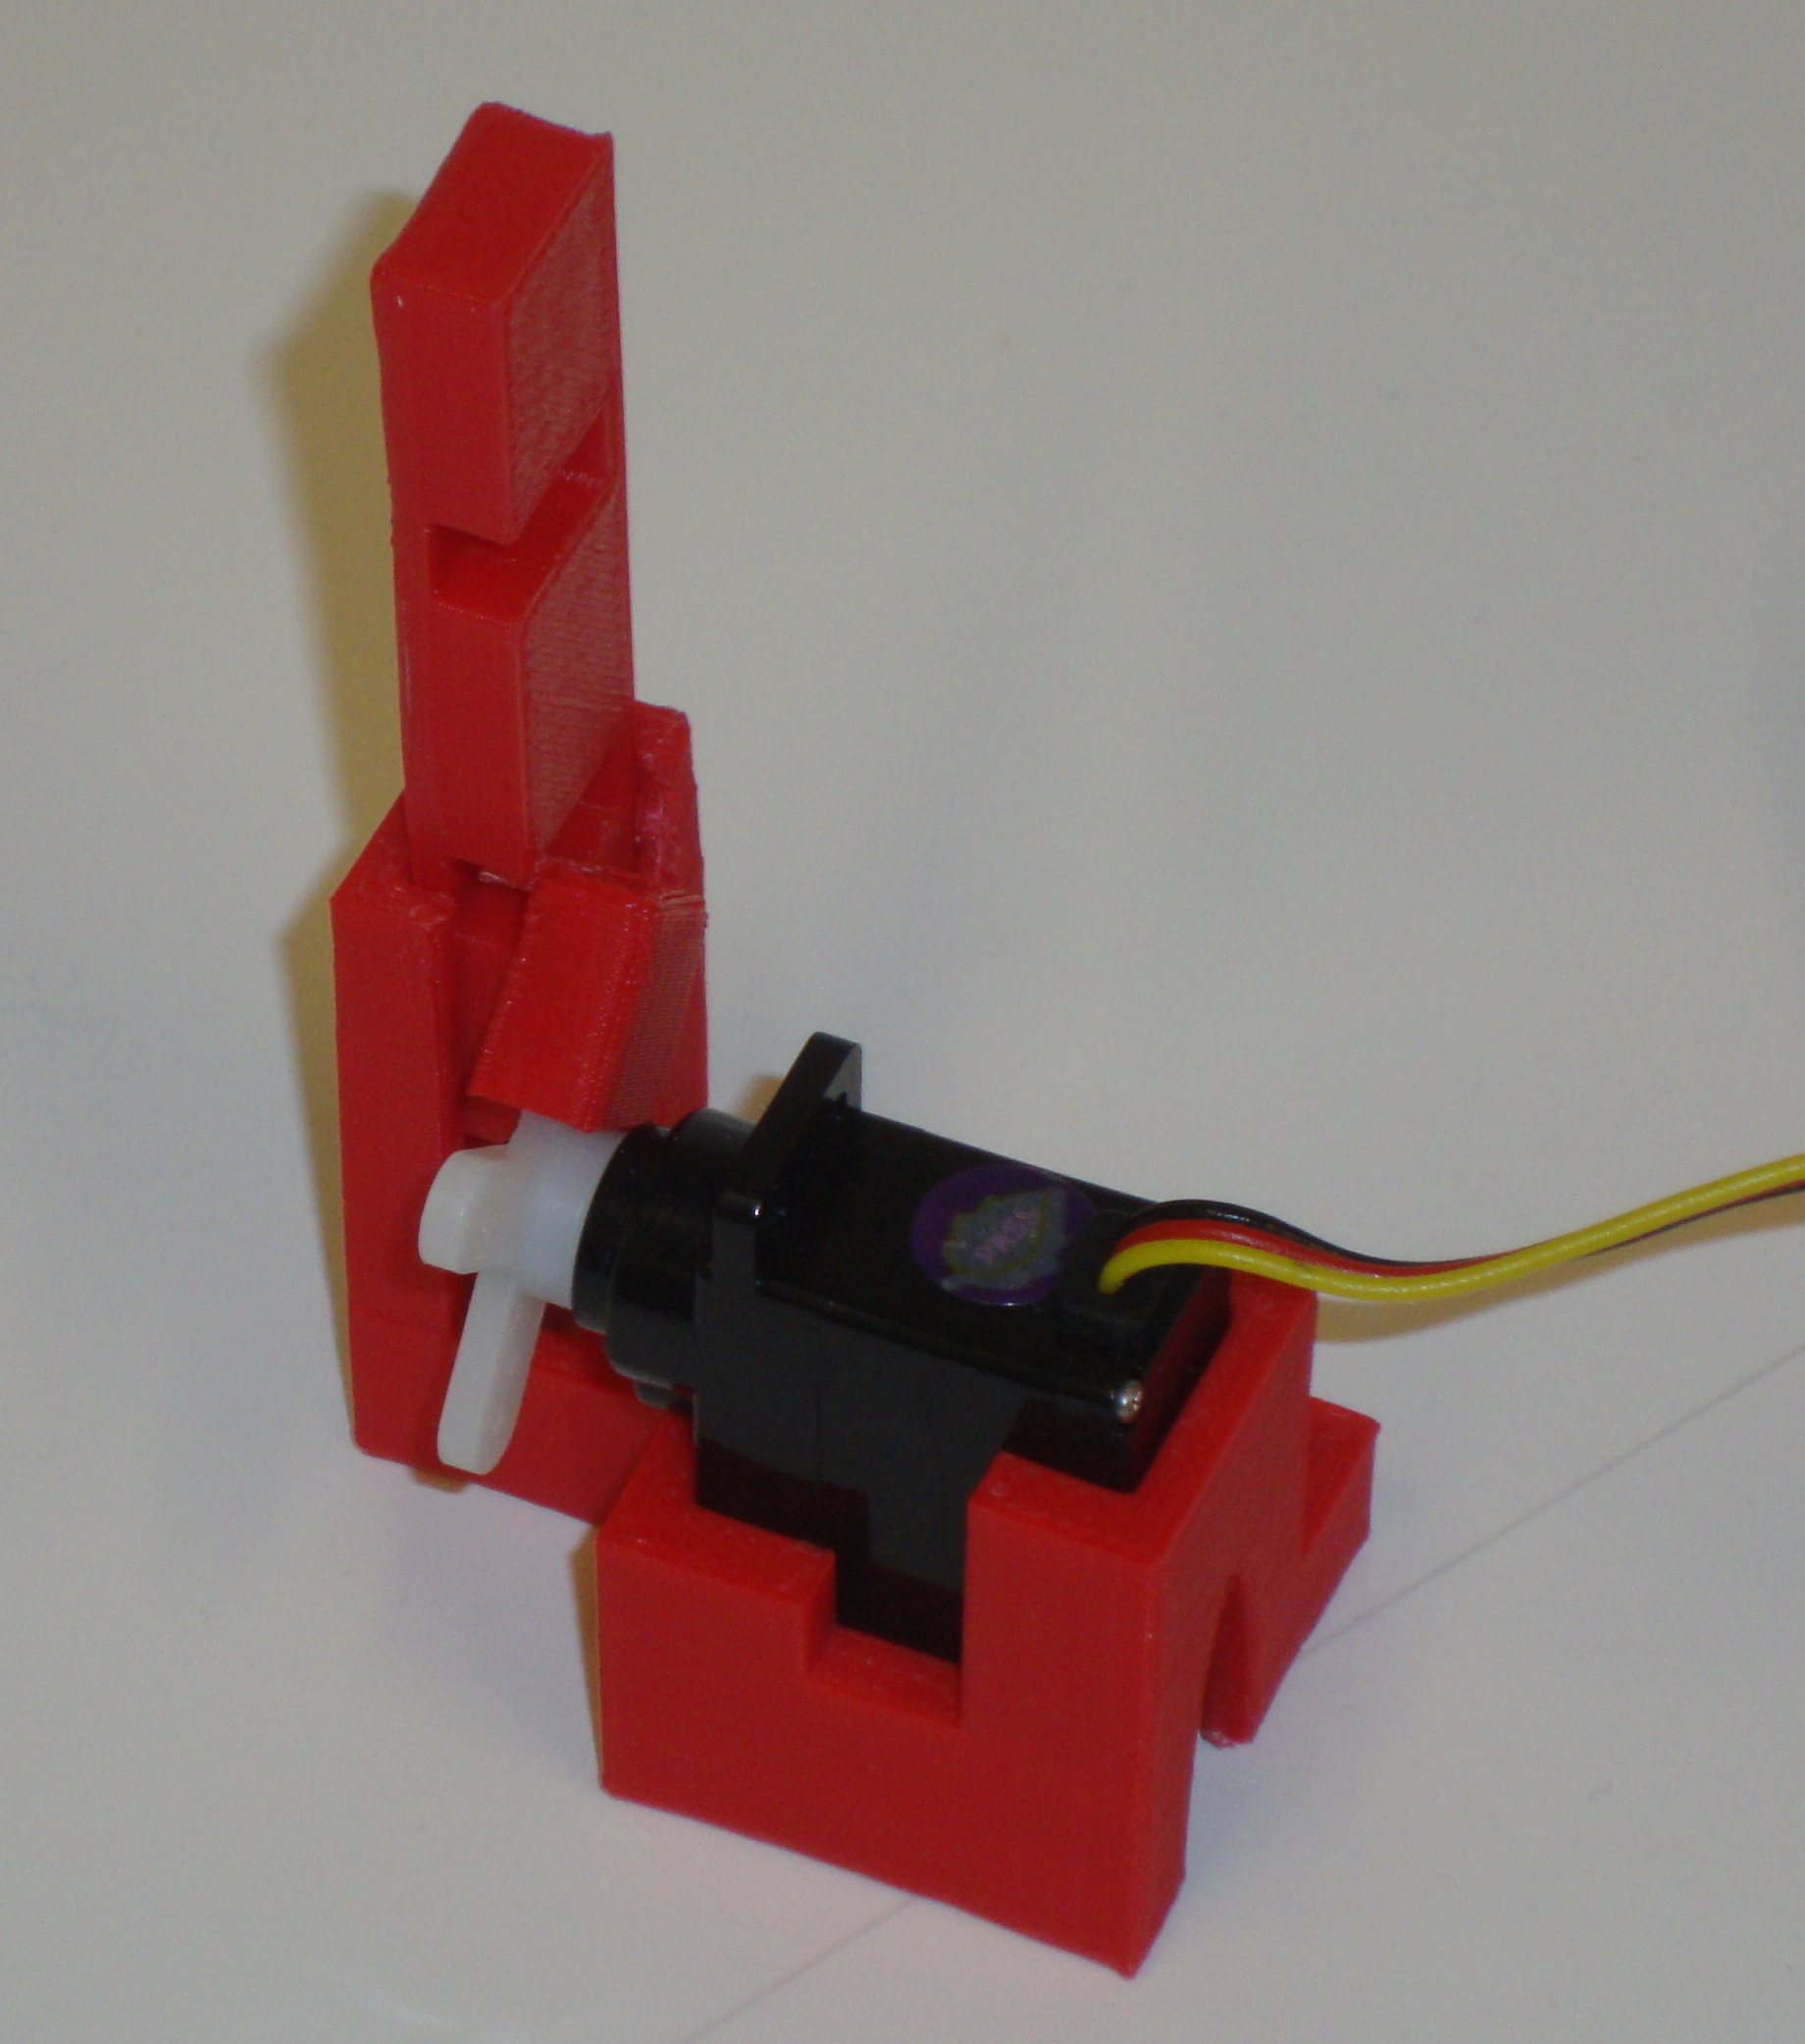
\includegraphics[width=\textwidth,height=\textwidth]{pos2.JPG}
                \caption{HaptiQ MaxPos}
                \label{fig:HaptiQ MaxPos}
        \end{subfigure}
        \caption{HTP and HaptiQ actuator mechanics}\label{fig:HTP and HaptiQ actuator mechanics}
\end{figure}

This version of the HaptiQ does not provide any case. The uneven surface leads to the lack of a reference point or plane for the actuators. This is a major problem in cases where the actuators change position while the user is not currently laying his hand on the device. In fact, it follows that when the blind user places the hand on top of the device again, he or her is not able to tell what the current state of the actuators is compared to the previous one. Two solutions are provided for the 4-HaptiQ: a mid-point reference and a plane reference static actuators (see Figure ~\ref{fig:HaptiQ reference static actuators}). It is not clear which type of reference actuator works best though. My hypothesis is that the plane reference actuator should be more comfortable when using the device and provides the same functionality than the point reference actuator. 

\begin{figure}
        \centering
        \begin{subfigure}[H]{0.5\textwidth}
                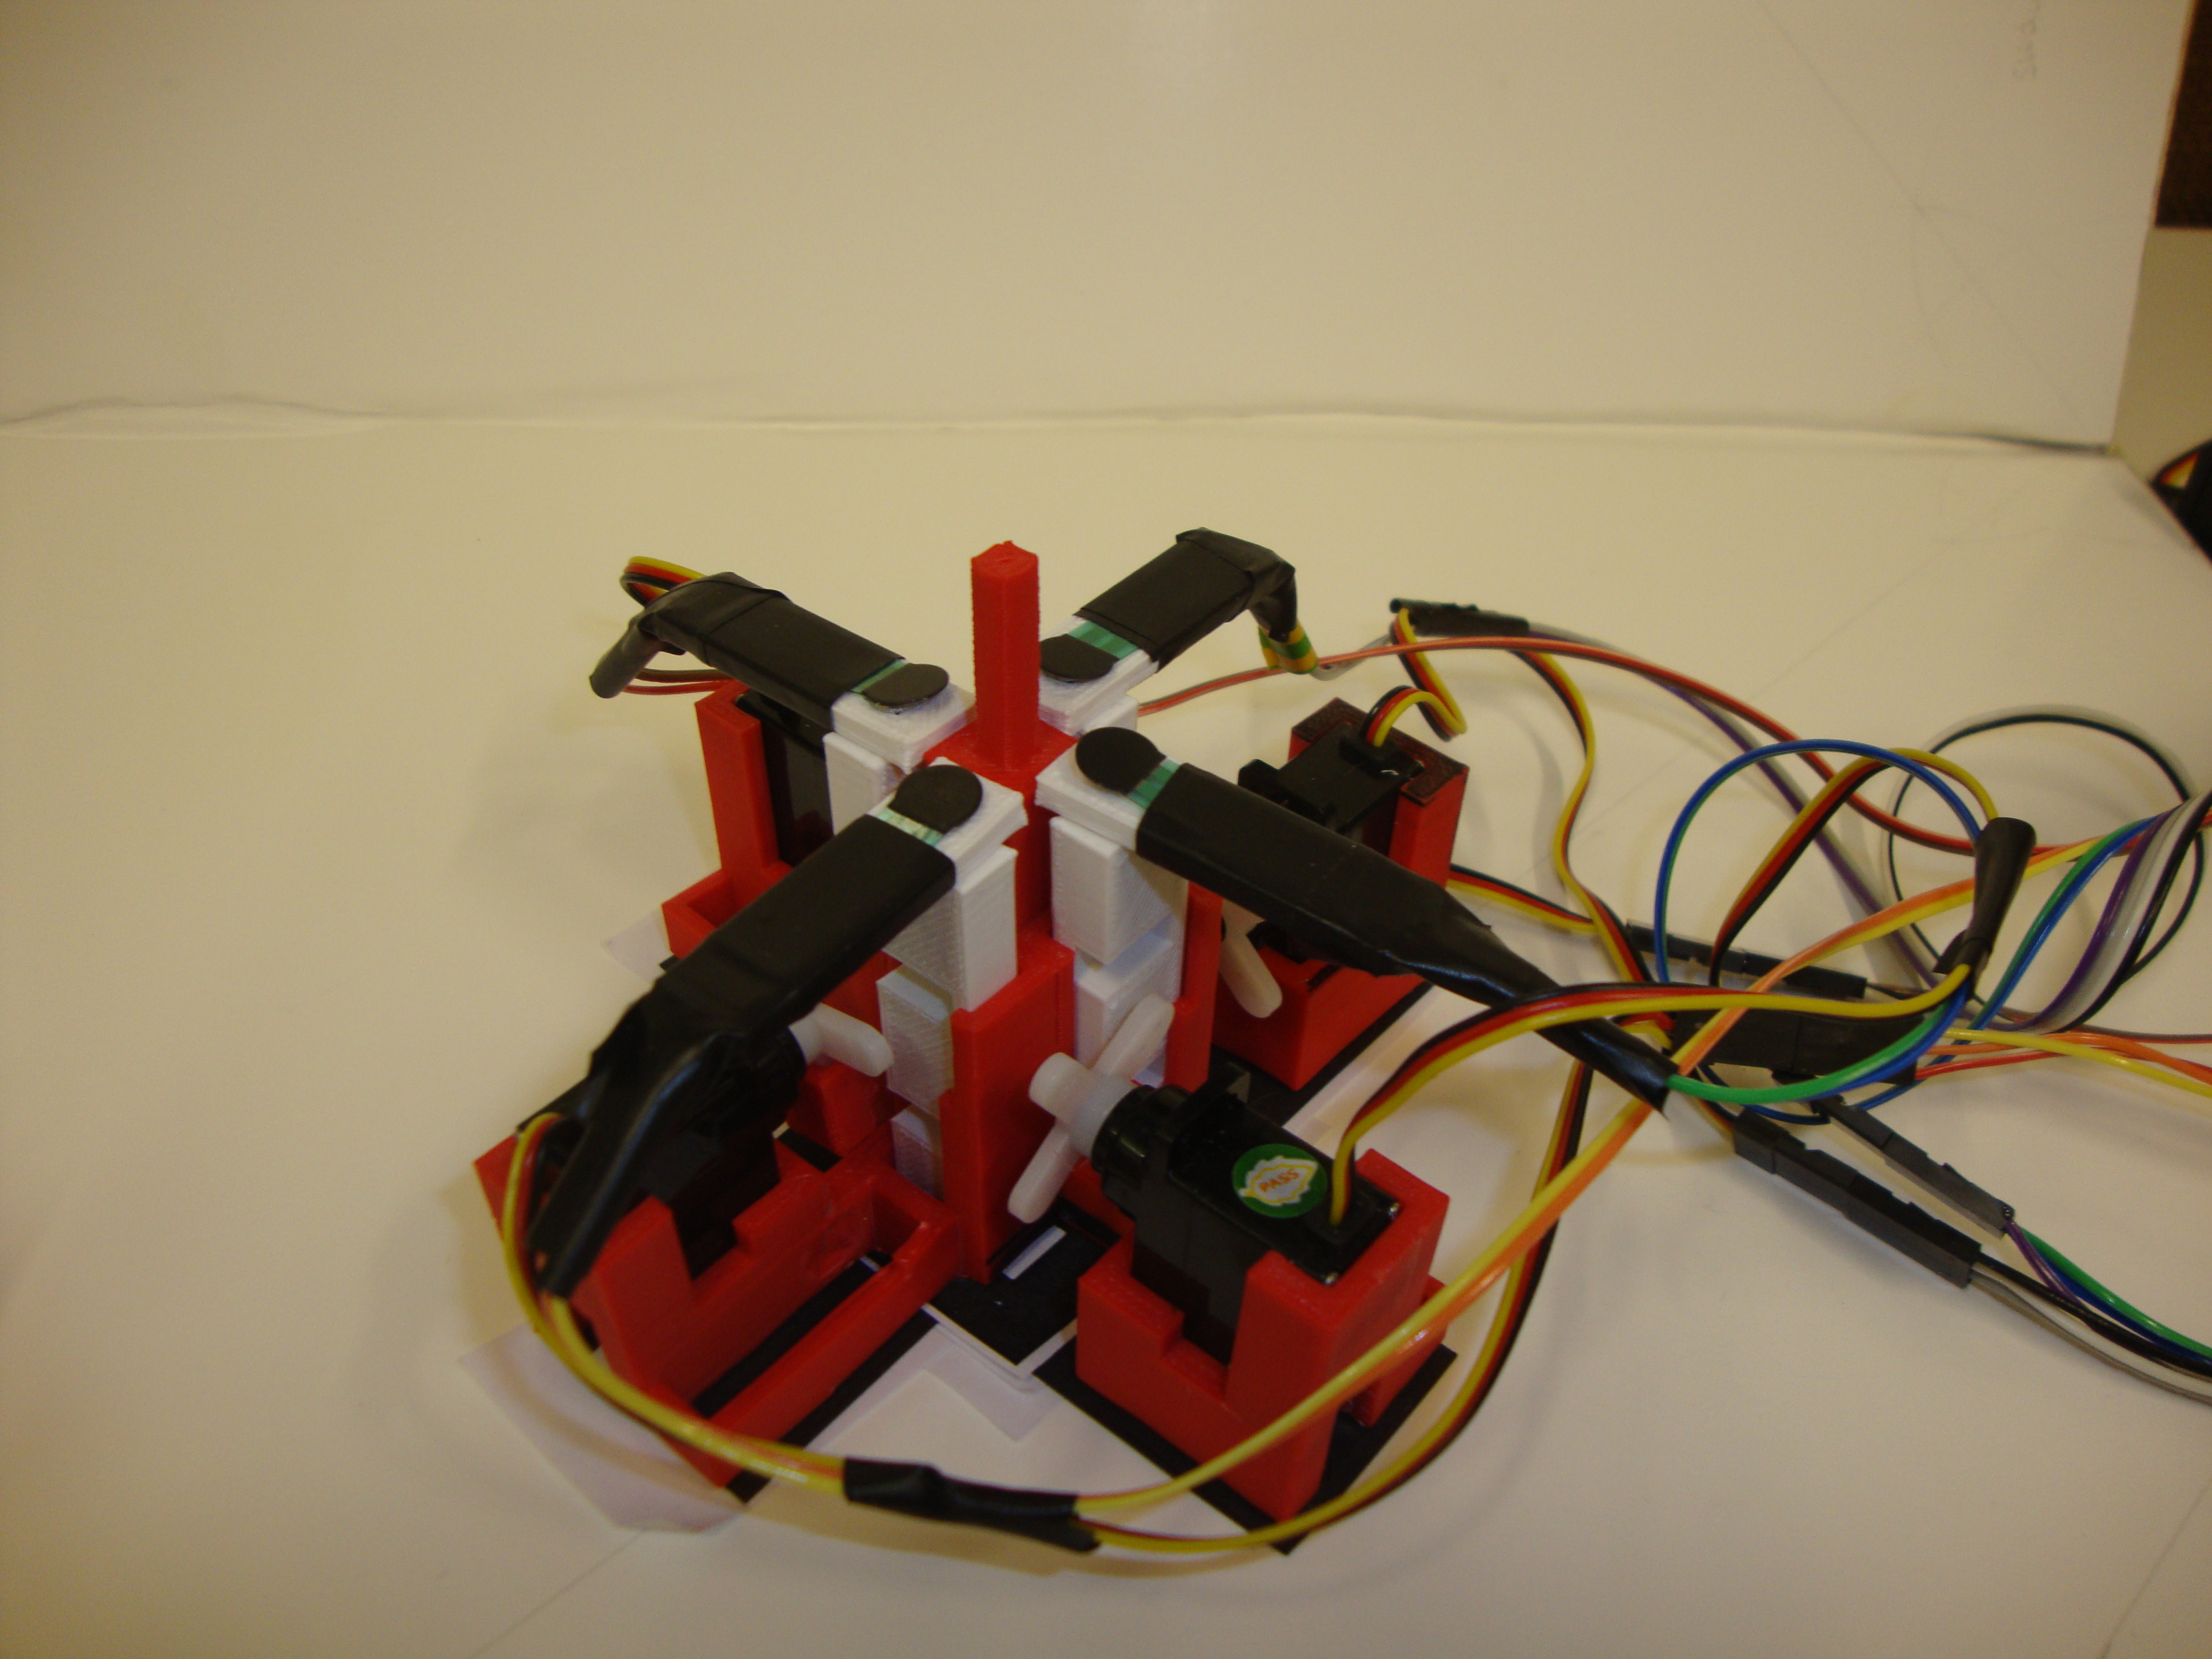
\includegraphics[width=\textwidth]{referencetype20.JPG}
                \caption{Mid-Point reference actuator}
                \label{fig:Mid-Point reference actuator}
        \end{subfigure}%
        ~ %add desired spacing between images, e. g. ~, \quad, \qquad etc.
          %(or a blank line to force the subfigure onto a new line)
        \begin{subfigure}[H]{0.5\textwidth}
                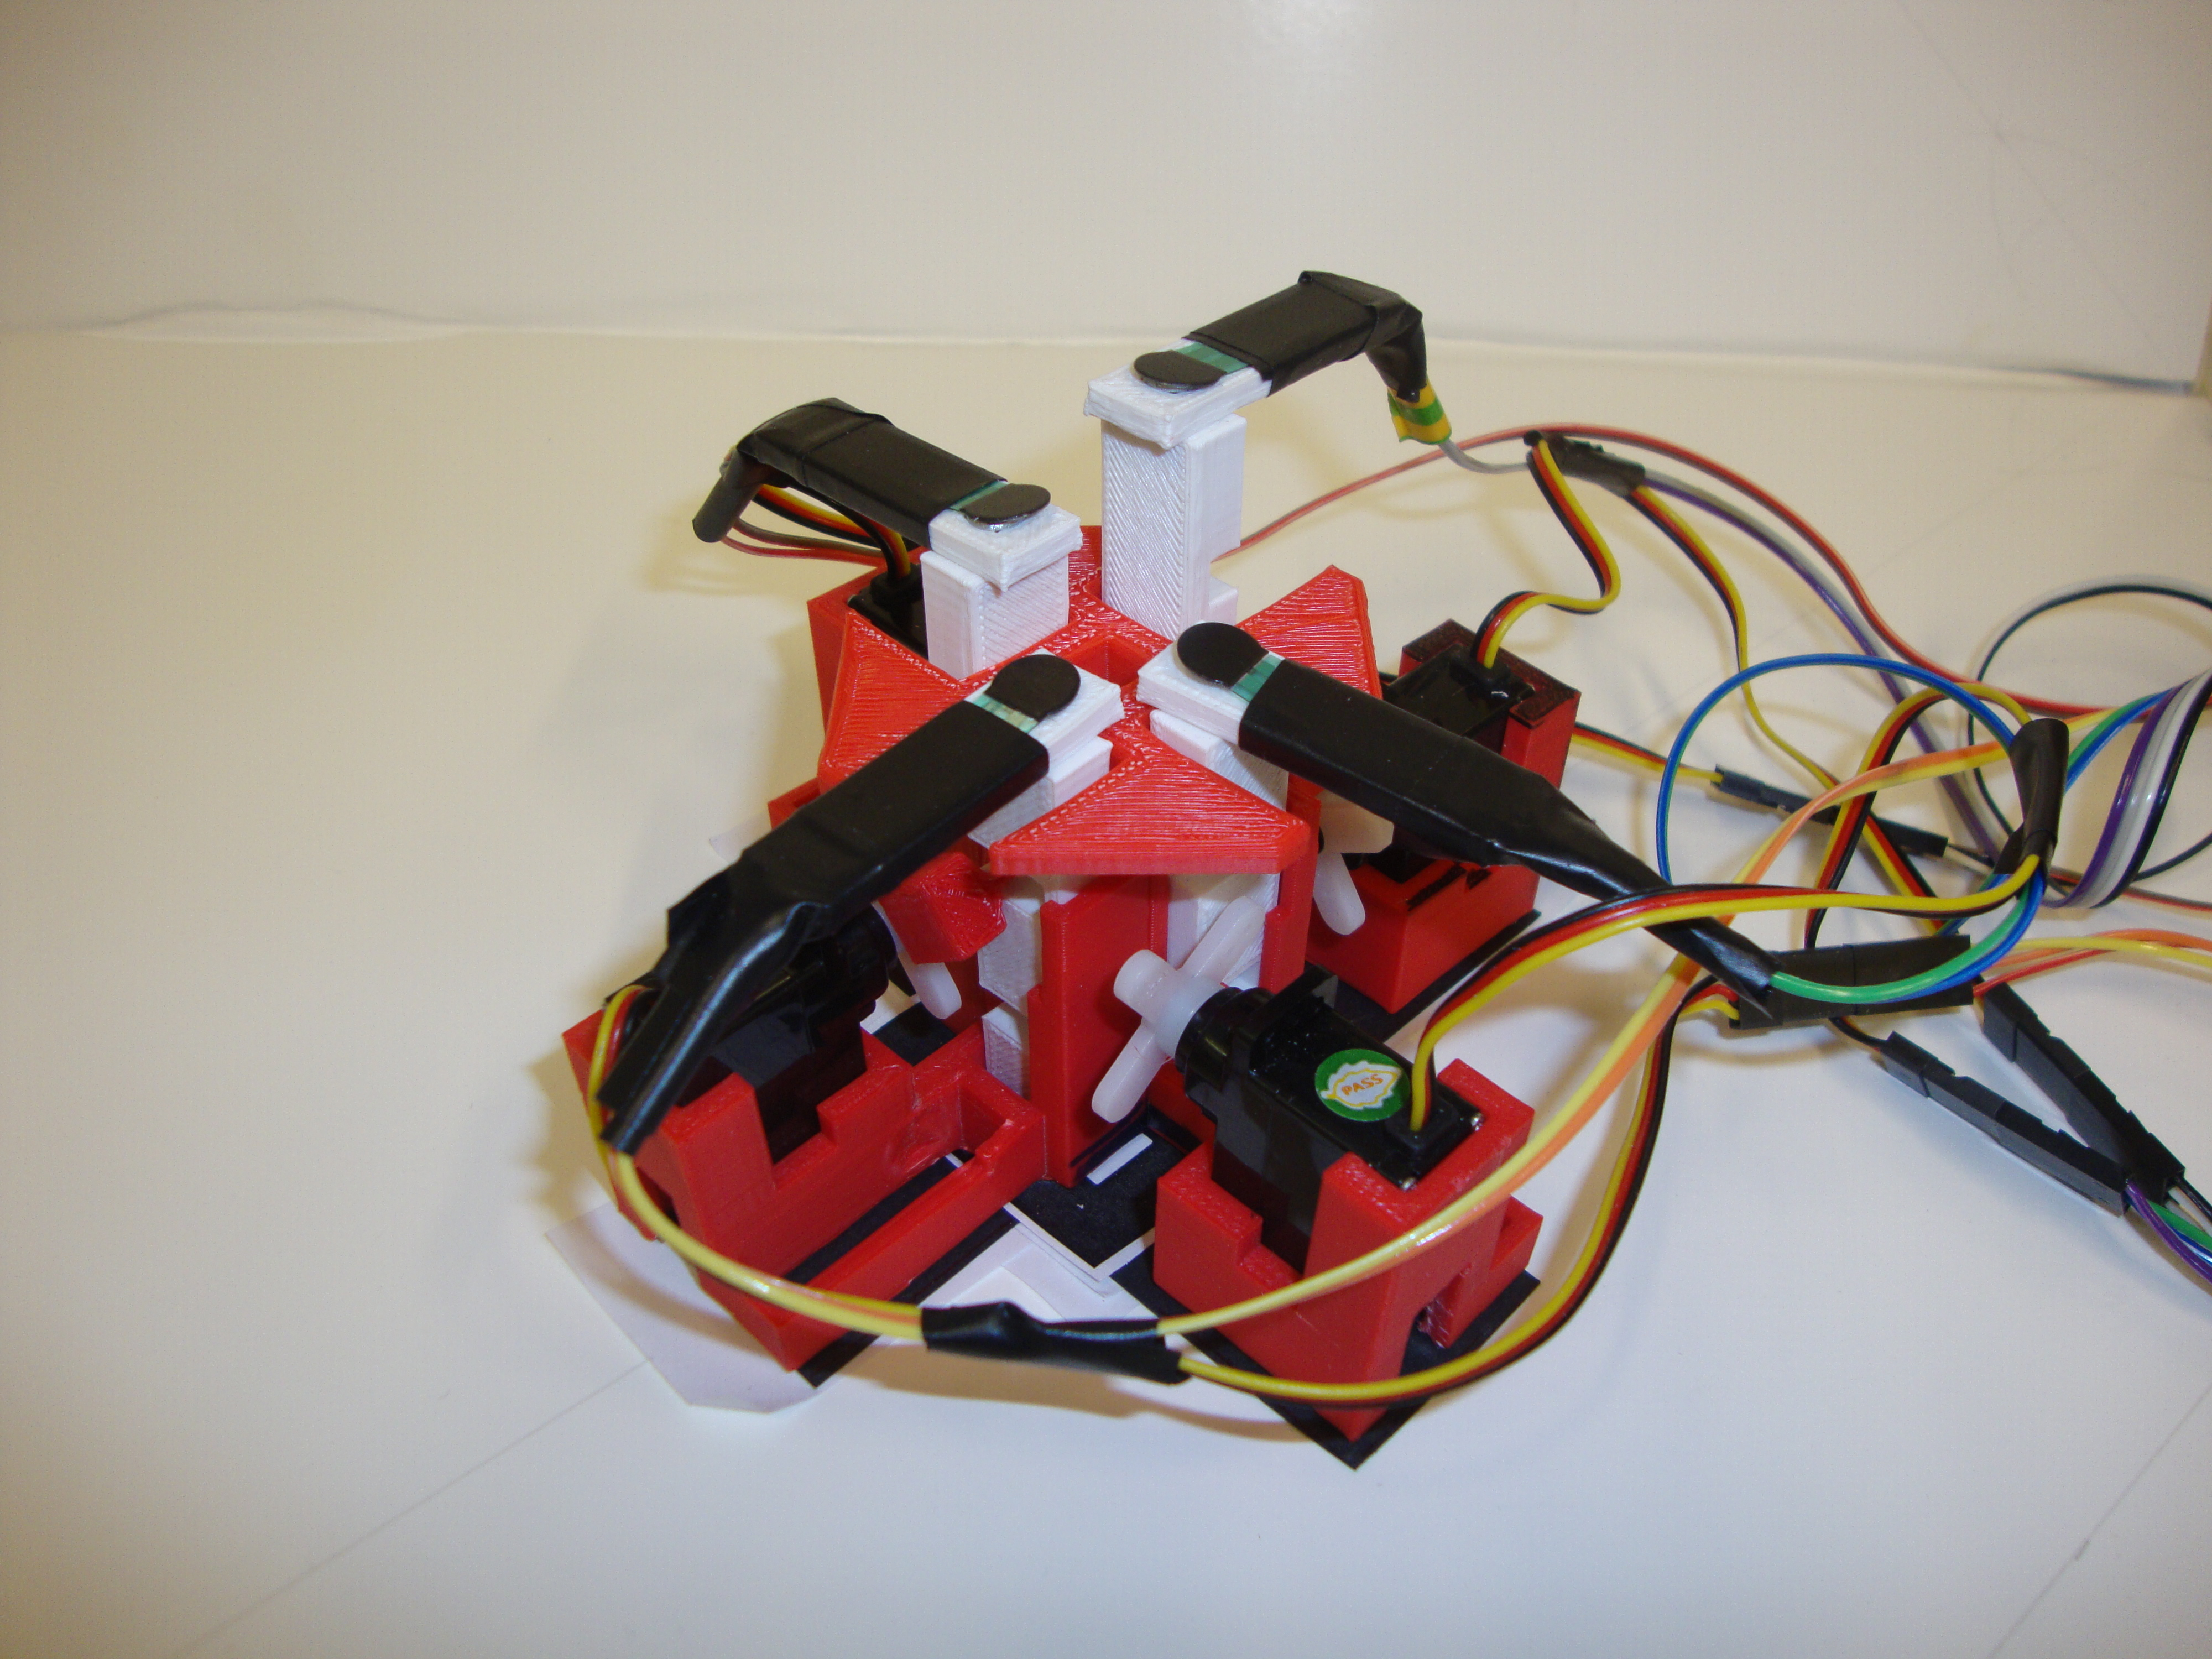
\includegraphics[width=\textwidth]{referencetype11.JPG}
                \caption{Plane reference actuator}
                \label{fig:Plane reference actuator}
        \end{subfigure}
        ~ %add desired spacing between images, e. g. ~, \quad, \qquad etc.
        \caption{HaptiQ reference static actuators}\label{fig:HaptiQ reference static actuators}
\end{figure}

The HaptiQ is the first vector-based display for blind users. Whether this design provides better feedback to users or not is unknown, because no study with participants could be conducted. Therefore, the actuators are designed so to support different tops in order to be able to evaluate the HaptiQ against a point-based haptic feedback TUI. In the version here presented, only vector-like tops are provided, but other type of tops can be easily printed and fasten to the actuators.   

Finally, the HaptiQ does not have any break to simulate friction. While it could be possible to add this feature, I decided that the primary goal of this project was just to focus on the vectorisation of the actuators. 

\subsection{8-HaptiQ}
The result of the final design iteration is the 8-HaptiQ. Using the same design of the 4-HaptiQ for eight actuators would lead to a considerable increase in size of the device. Therefore, the 8-HaptiQ has been completely re-engineered (see Figure ~\ref{fig:8-HaptiQ}). 

\begin{figure}[H]
  \centering
  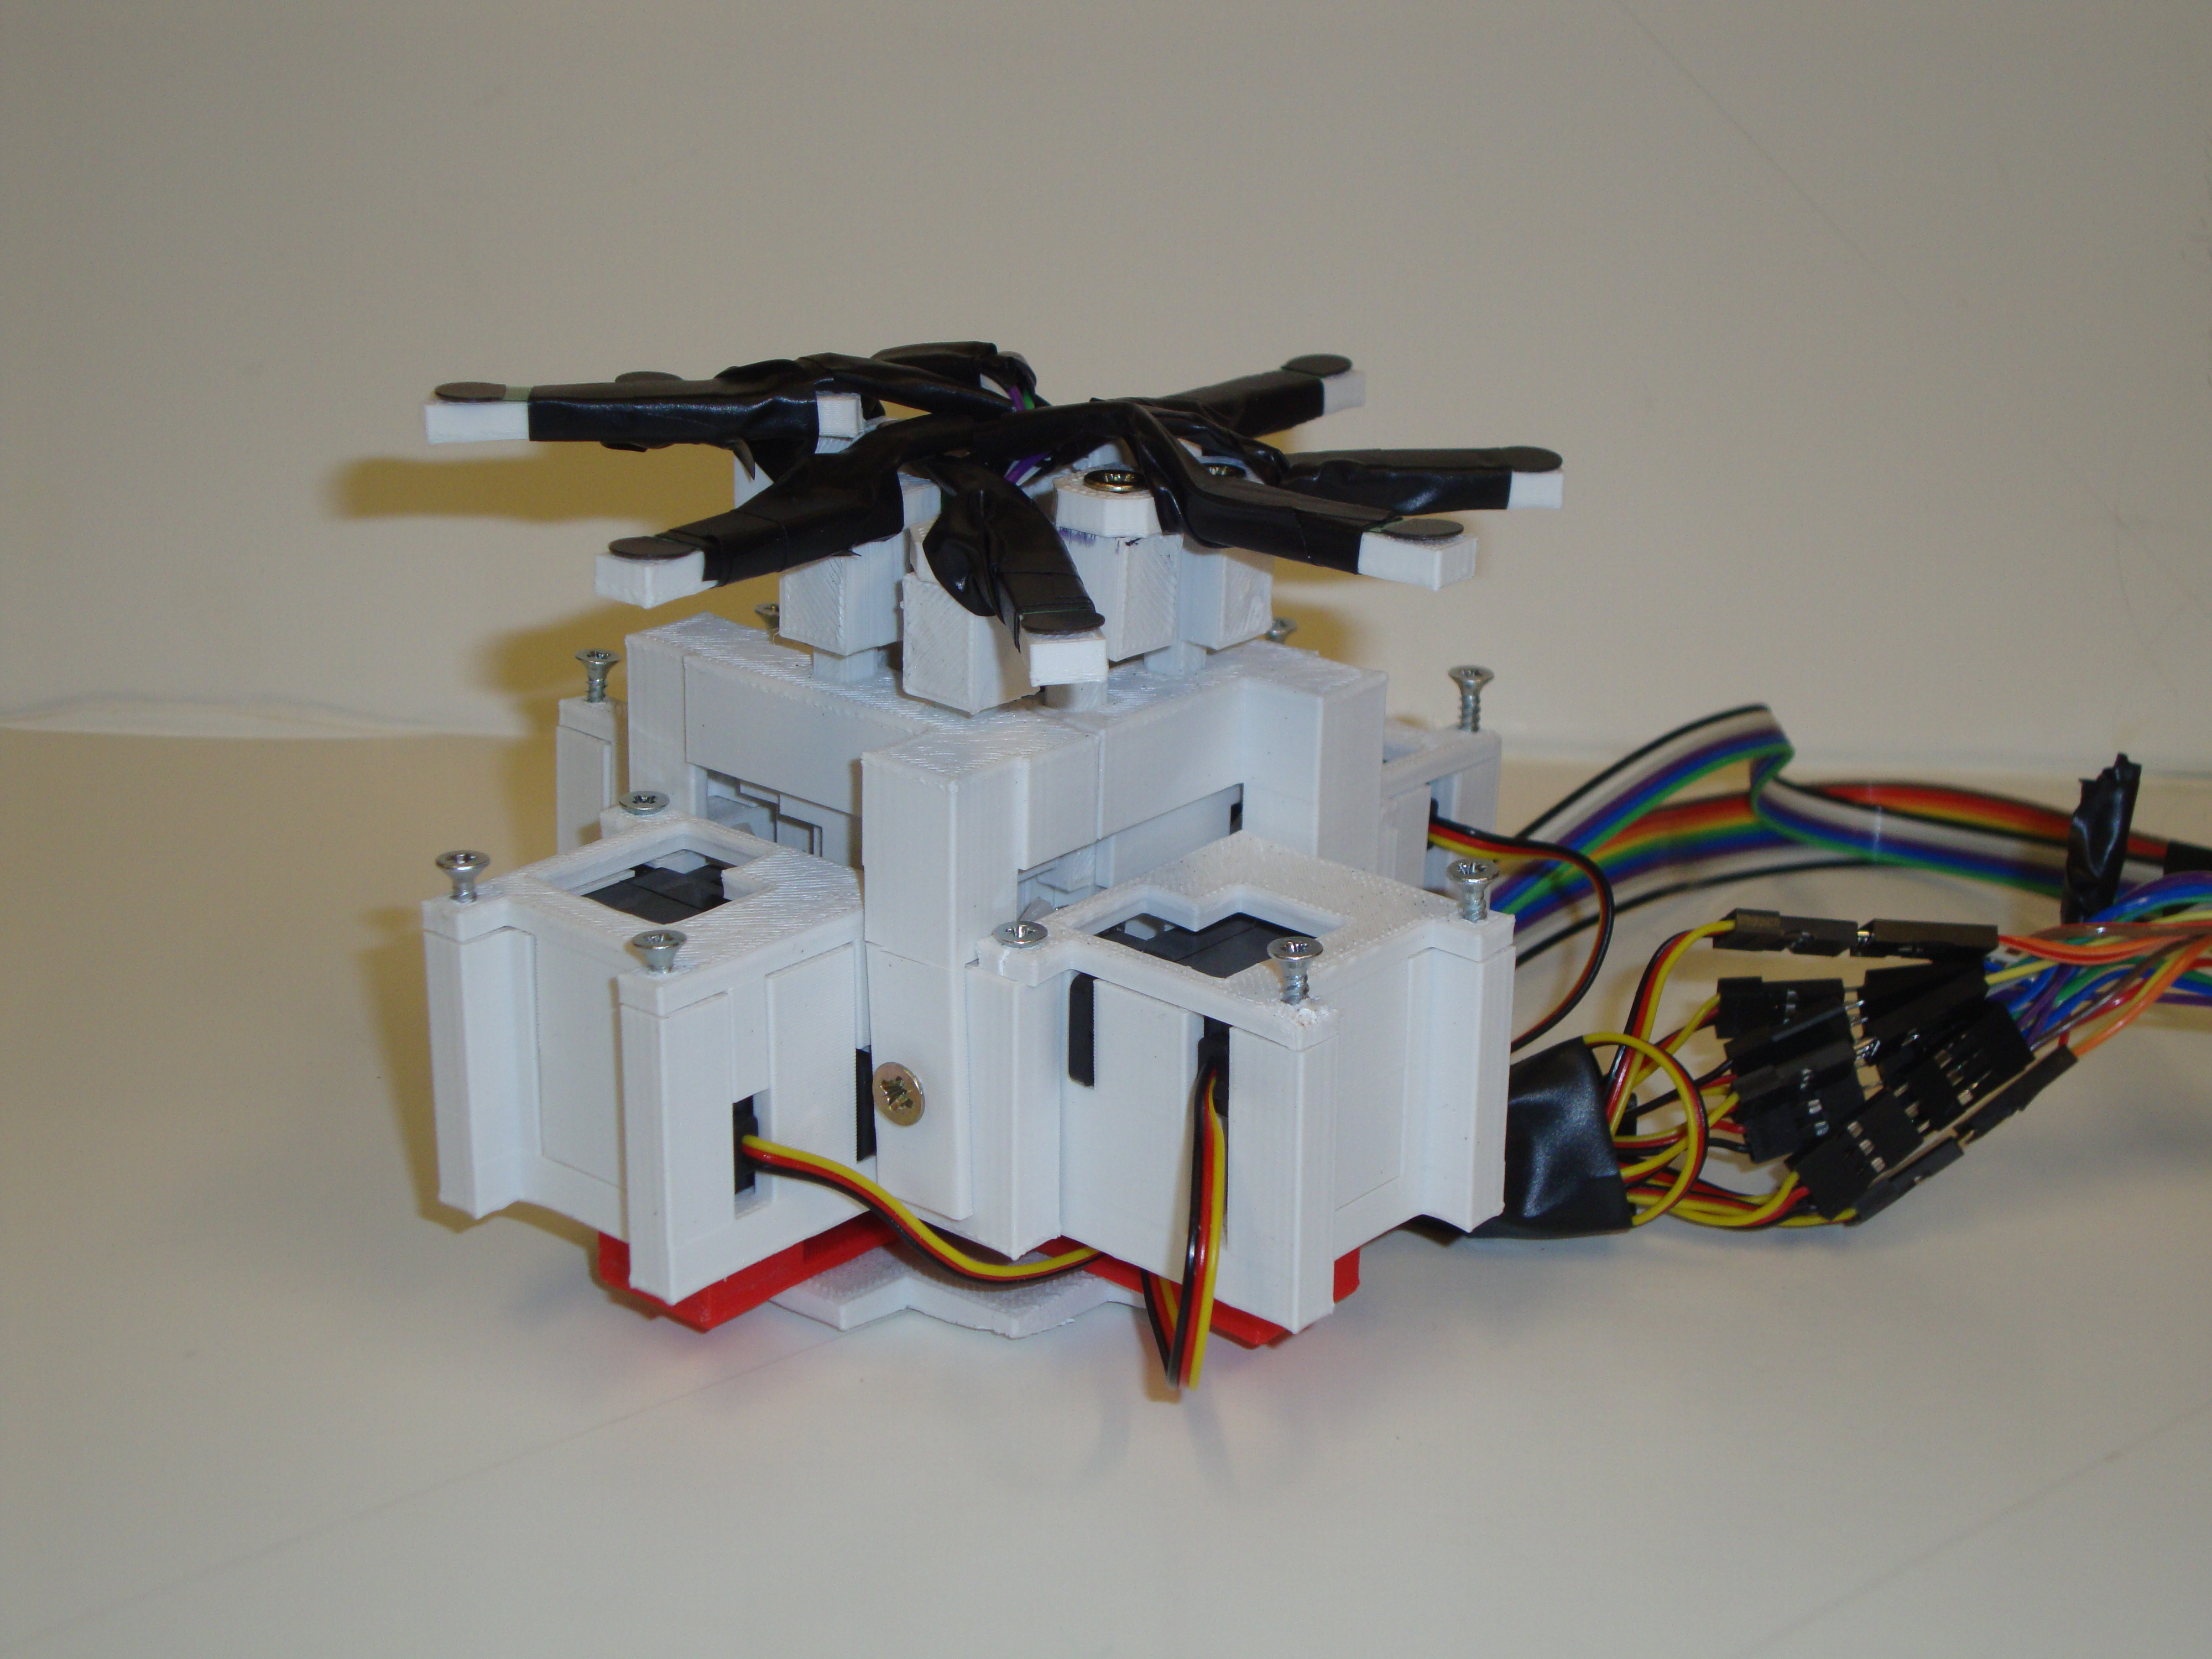
\includegraphics[width=0.7\textwidth]{HaptiQ1.JPG}
  \caption{8-HaptiQ}
  \label{fig:8-HaptiQ}
\end{figure}

The 4-HaptiQ not only is not optimised in terms of space, but its wiring is also not well engineered. As it is possible to observe in figure ~\ref{fig:HaptiQ reference static actuators} the wiring does not allow the device to be used comfortably, especially when one wants to rotate it. 
The servos in the 8-HaptiQ are organised in couples. Unlike its predecessor, the servos are positioned horizontally (see Figure \missingfigure{picture of two servos bla bla bla}) and the screws are moved more toward the center of rotatory mechanism of the servos. These design choices allow the device to be more compact and still preserve the same functionalities of the 4-HaptiQ. 
The device is lift up by an additional structure laying below it, allowing the wiring to be less disruptive. 

With the gathering of the wires for the sensors to the center of the device, the position of the sensors is also inverted compared to the 4-HaptiQ. While in the 4-HaptiQ these were meeting in the middle, with this new version of the HaptiQ the sensors are spread to the outside. It is not clear whether this design choice is an advantage or not in terms of usability. Alternatives to this solution will be provided in the near future, as discussed in the Future Work chapter.

The 8-HaptiQ takes a different approach for the design of the actuators guides. In the first version, a base was provided for the actuator, which limits this to move further down when this is at its minimum position (see Figure ~\ref{fig:HaptiQ MinPos}). But to provide an optimal wiring, the 8-HaptiQ combines the guides for all the actuators with the reference plane (see Figure \missingfigure{add sketchup screenshot}). Additional connecting screws alow the actuators to be always controlled by the servos and not to fall below its minimum position. 

\section{The API}

This section discusses the design choices for the API for the HaptiQ. The general idea behind the HaptiQ API is similar to the HapticTouch toolkit \cite{ledo2012haptictouch}. However, this has been completely redesigned to support:

\begin{itemize}
	\item multiple actuators
    \item multiple pressure sensors
    \item a completely new approach to HapticObjects and HapticBehaviours
    \item actions called when input is received by the user
    \item additional API to get input position of the device from different hardware
\end{itemize}

Each of these will be discussed in the following sections. 

\subsection{Overall Structure}

The API consists of two main components: the HaptiQ API used to control the device and the Input API (see Figure ~\ref{fig:api}). 
The HaptiQ API component is designed to provide high and low access to the HaptiQ. This allows the API to be versatile and to be used by beginner, intermediate and advanced developers. 
The HaptiQ API retrieves the position of the device through the Input API. 

The following two sections describe these components in more details.

\begin{figure}[H]
  \centering
  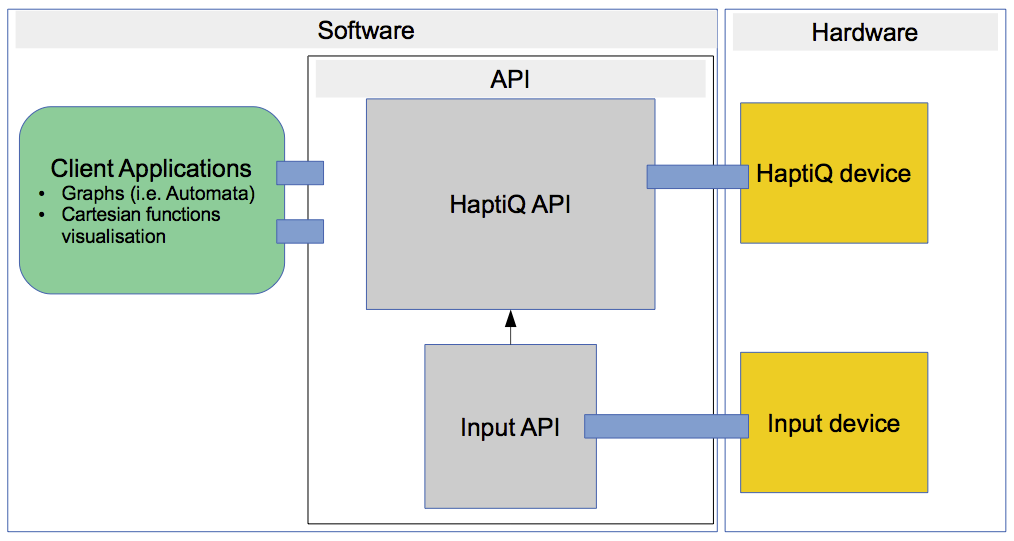
\includegraphics[width=1.0\textwidth]{General_overview.png}
  \caption{API General Overview}
  \label{fig:api}
\end{figure}

\subsection{Input API}

Initially, the HaptiQ, like the HTP, was designed to work on a Microsoft PixelSense table \cite{pixelsense}.
Microsoft Surface Bytetags are located underneath the HTP to get the location of the device in the table. However, official Bytetags are expensive and printing them with a normal printer does not lead to satisfying results. In addition, the HaptiQ will be used in the near future on digital tables that do not support the Surface SDK. Therefore, in order to abstract the HaptiQ API from any hardware input dependence, a separate API component has been created (see Figure ~\ref{fig:input_api}). 

The architectural structure of the Input API is based on the classic Factory pattern. This adds a level of abstraction over the hardware that should be used to get the position of the HaptiQ. Currently the API supports Bytetags and Glyphs recognition \todo[noline]{add reference}. But client applications can also add their own customised class to support different position detection methods. 

\begin{figure}[H]
  \centering
  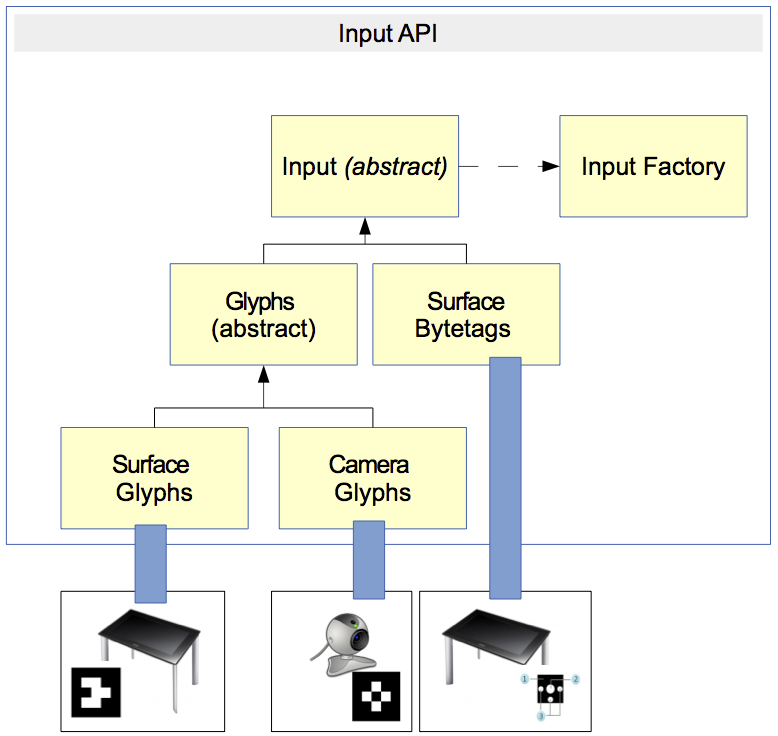
\includegraphics[width=0.5\textwidth]{input.png}
  \caption{Input API}
  \label{fig:input_api}
\end{figure}

\subsection{HaptiQ API}

The HaptiQ API is the central component of the API, which connects the Input API, the HaptiQ device and the client applications together (see Figure ~\ref{fig:haptiQ_api}). 

\begin{figure}[H]
  \centering
  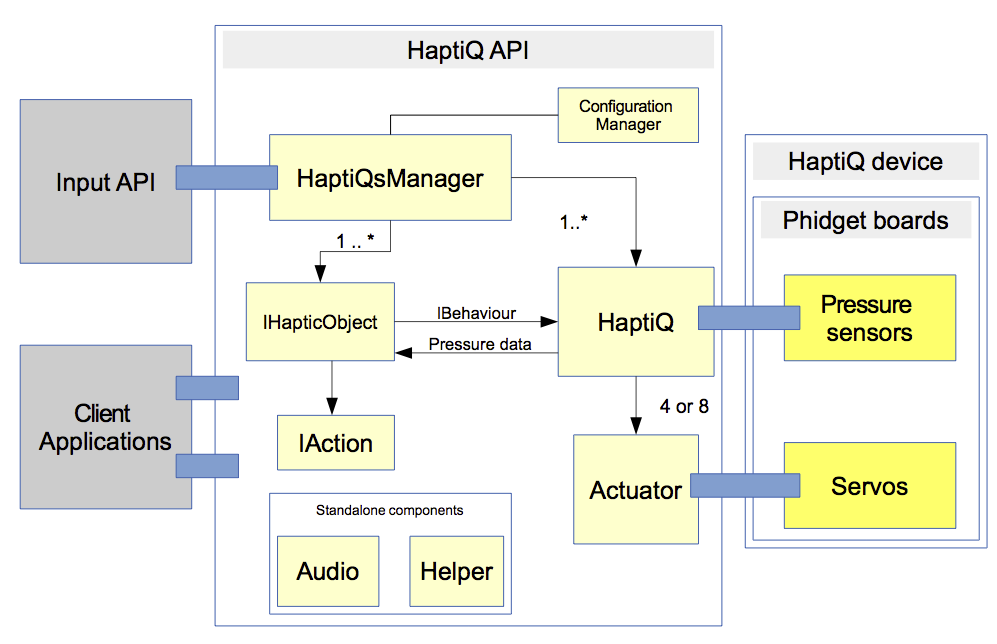
\includegraphics[width=1.0\textwidth]{haptiQAPI.png}
  \caption{HaptiQ API}
  \label{fig:haptiQ_api}
\end{figure}

\subsubsection{Haptic Objects}
Basic haptic objects are provided by the API, to be used easily by WPF applications. The main focus of such applications should be the information one wants to convey, rather than its aesthetics. Therefore, only simple shapes are provided. Obviously, one can extend the HapticShape abstract class to provide more interesting shapes.

It is possible to register an action per object, which gets called whenever input is received from the device through the pressure sensors. 

\missingfigure{add screen shot of all haptic objects}

\begin{itemize}
	\item circle
    \item rectangle
    \item link
    \item line
    \item polyline
\end{itemize}

\subsubsection{Speech Synthesizer}

The Speech Synthesizer is a standalone subcomponent of the HaptiQ API which allows any part of the API, as well as client applications, to output textual information as audio, provided that the machine has a sound card.

While this is a small component, it still plays an important role in the API. Ungar and Blades \cite{ungar2000can} discuss whether the conjoint retention hypothesis, combining spatial and linguistic information, can provide richer haptic cueing. Their study did not show any significant improvement when adding audio feedback. However, they results were not definitive. Therefore, I decided to follow the trend of many commercial applications, like VoiceOver, which use audio to provide textual and position feedback too.

\section{Tactons}

Pietrzak et al. \cite{pietrzak2009creating} propose a set of tactons that can be used on pin array devices and that could be used to indicate edgs and directions. These tactons are designed for a 4x4 pins grid. The HaptiQ provides a maximum of eight actuators, uses lines rather than points to convey haptic cues and can provide height information as well (pin arrays typically provide only 0/1 information). Here, I present a new set of tactons.

A tacton, or behaviour, is used by an HapticObject to notify a device how to react when this is located on top of it. In the provided API there is a strong relationship between each HapticObject and a behaviour. Nonetheless, behaviours can be used by client defined HapticObjects or directly from a client application.

In the following sections, the scale in figure ~\ref{fig:scales} will be used to represent the heights of the actuators \todo[noline]{invert the scales?}.

\begin{figure}[H]
  \centering
  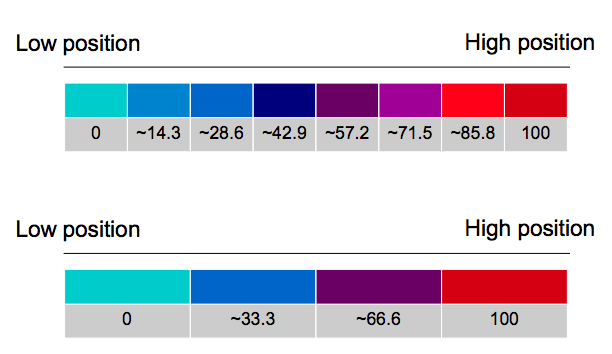
\includegraphics[width=0.6\textwidth]{scales.png}
  \caption{Blue-Red scale used to indicate the height of the actuators for the 4/8-HaptiQ tactons. Values represent the positions of the actuators in percentage.}
  \label{fig:scales}
\end{figure}

\subsection{Flat and Max}

Flat and Max are the simplest tactons of the set (see Figure ~\ref{Basic tactons}). The Flat tacton is typically used to indicate that underneath the device there are no objects or information. The Max behaviour, instead, can be used to represent the existance of an object. For instance, when the device is inside an HapticRectangle the Max behaviour is played. 

\begin{figure}[H]
  \centering
  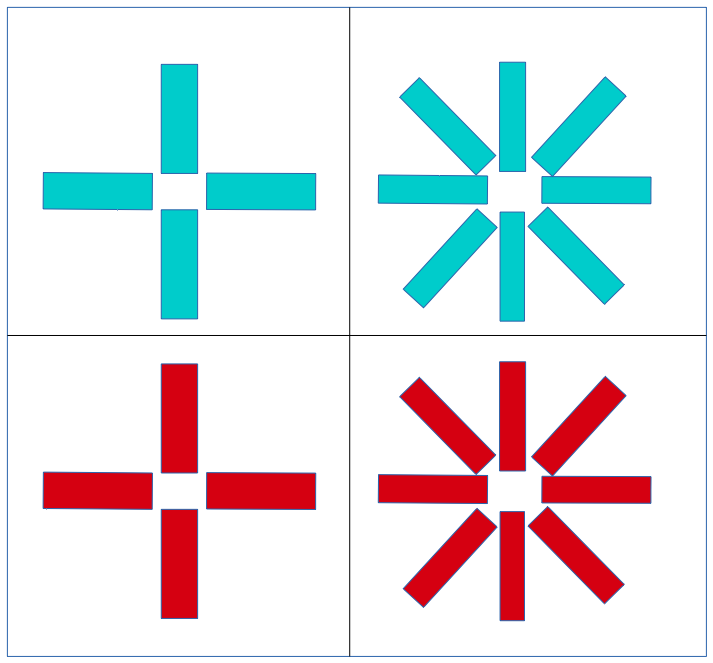
\includegraphics[width=0.5\textwidth]{basic.png}
  \caption{Basic tactons: Flat and Max}
  \label{fig:Basic tactons}
\end{figure}

\subsection{Notification}

The Notification tacton, similarly to the Max tacton, can also be used to notify an object. In the case being, this tacton is used to notify an HapticCircle. This tacton consists into cyclically change the positions of the actuators (see Figure ~\ref{fig:notification}). 

\begin{figure}[H]
        \centering
        \begin{subfigure}[H]{0.5\textwidth}
                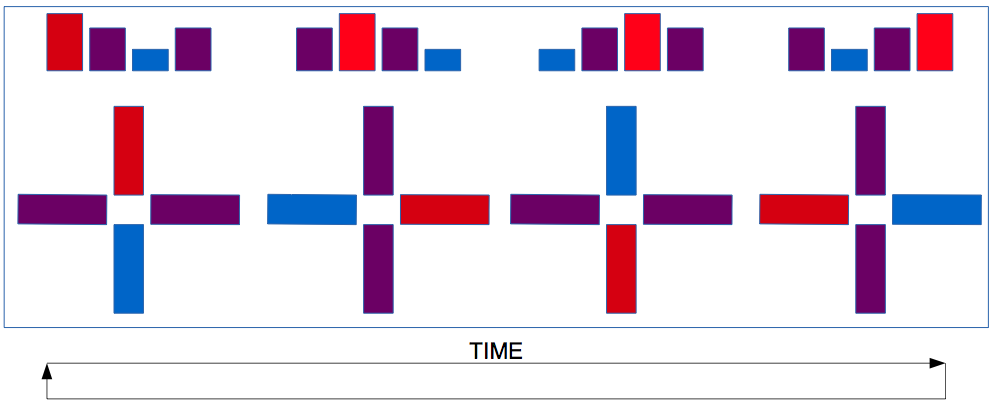
\includegraphics[width=\textwidth]{notification-4.png}
                \caption{4-HaptiQ}
                \label{fig:notification-4}
        \end{subfigure}%
        ~ %add desired spacing between images, e. g. ~, \quad, \qquad etc.
          %(or a blank line to force the subfigure onto a new line)
        \begin{subfigure}[H]{0.5\textwidth}
                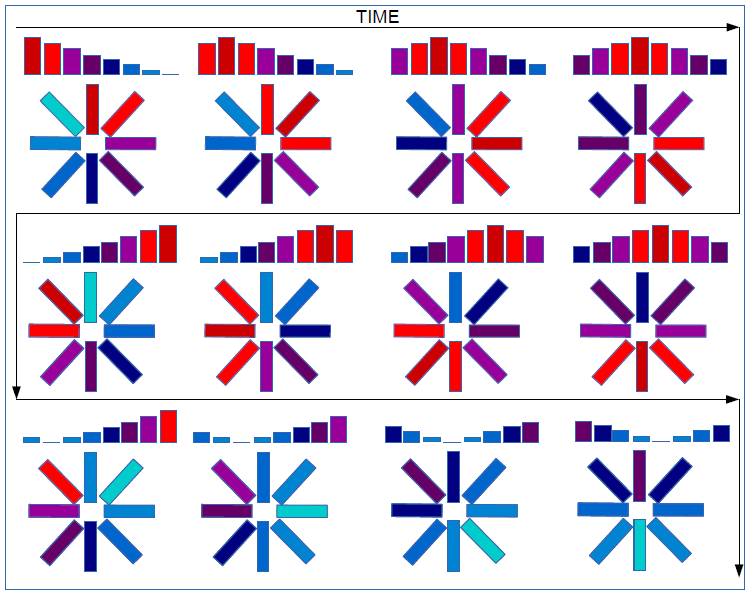
\includegraphics[width=\textwidth]{notification-8.png}
                \caption{8-HaptiQ}
                \label{fig:notification-8}
        \end{subfigure}
        ~ %add desired spacing between images, e. g. ~, \quad, \qquad etc.
        \caption{Notification tacton}\label{fig:notification}
\end{figure}

\subsection{Direction}

The Direction tacton \todo[noline]{rename to edge?} is probably the most significant one of all the tactons. This allows the HaptiQ to represent edges and corners. 

Figure ~\ref{fig:edges} show how the combinations of actuators, in both the prototypes, are used to represent edges. The resolution of the device is increased by alternatively actuating adjacent actuators. It is possible to achieve a precision of 45° and 22.5° for the 4-HaptiQ and the 8-HaptiQ respectively. 

\begin{figure}[H]
        \centering
        \begin{subfigure}[H]{0.3\textwidth}
                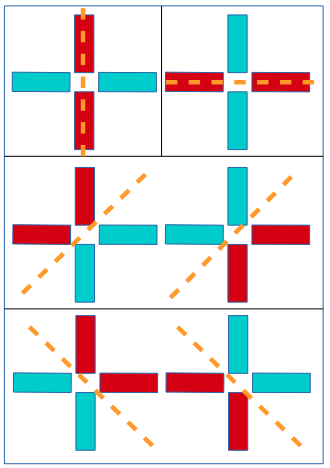
\includegraphics[width=\textwidth]{direction-4.png}
                \caption{4-HaptiQ}
                \label{fig:direction-4}
        \end{subfigure}%
        ~ %add desired spacing between images, e. g. ~, \quad, \qquad etc.
          %(or a blank line to force the subfigure onto a new line)
        \begin{subfigure}[H]{0.5\textwidth}
                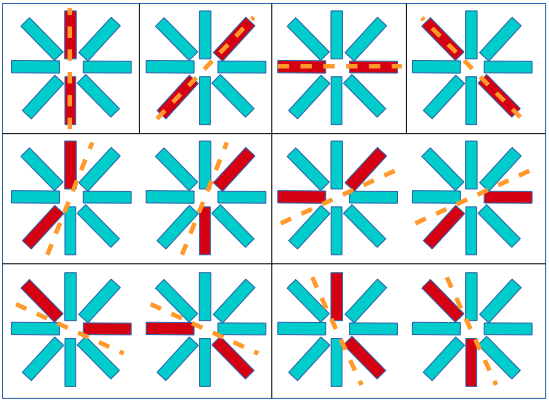
\includegraphics[width=\textwidth]{direction-8.png}
                \caption{8-HaptiQ}
                \label{fig:direction-8}
        \end{subfigure}
        ~ %add desired spacing between images, e. g. ~, \quad, \qquad etc.
        \caption{Direction tacton - Edges}\label{fig:edges}
\end{figure}

It is also possible to represent corners, which are merely the combinations of two edges. The 4-HaptiQ can represent corners of 90° with a precision of 45° (see Figure ~\ref{fig:corner-4}). Indeed, the 8-HaptiQ can represent corners of 45°, 90° and 135°, with a precision of 22.5° (see Figures ~\ref{fig:corner-8}, ~\ref{fig:corner-8c}). 

\begin{figure}[H]
        \centering
        \begin{subfigure}[H]{0.5\textwidth}
                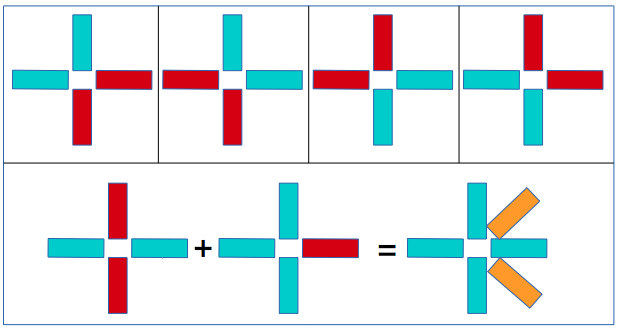
\includegraphics[width=\textwidth]{corners-4.png}
                \caption{4-HaptiQ}
                \label{fig:corner-4}
        \end{subfigure}%
        ~ %add desired spacing between images, e. g. ~, \quad, \qquad etc.
          %(or a blank line to force the subfigure onto a new line)
          
        \begin{subfigure}[H]{0.4\textwidth}
                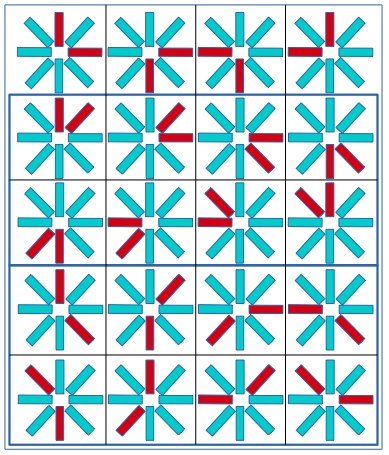
\includegraphics[width=\textwidth]{corners-8.png}
                \caption{8-HaptiQ}
                \label{fig:corner-8}
        \end{subfigure}
        ~ 
         \begin{subfigure}[H]{0.4\textwidth}
                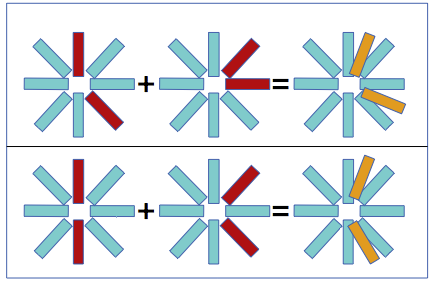
\includegraphics[width=\textwidth]{corners-8c.png}
                \caption{8-HaptiQ (combinations)}
                \label{fig:corner-8c}
        \end{subfigure}
        ~ %add desired spacing between images, e. g. ~, \quad, \qquad etc.
        \caption{Direction tacton - Corners}\label{fig:corners}
\end{figure}

The Direction tacton is used by the HapticRectangle, to represent its borders, and the HapticLine and HapticPolyline objects. 

\subsection{Pulsation and Linear}
The Pulsation and Linear tactons are used with the HapticLink to represent the sign of the link between two Haptic objects. Figure ~\ref{fig:pulsation} shows two cases of the pulsation tacton for the 4-HaptiQ. By symmetry it is possible to represent 8 (or 16 for the 8-HaptiQ) directions. This tacton also allows frequency to be specified, so that pulsation increases as one gets closer to the target. 

The Linear tacton, on the other hand, is the union of the pulsation tactons with not pulsation. One can also specify a linear factor, so that the height of the actuators increases linearly as one gets closer to the target. 

\begin{figure}[H]
  \centering
  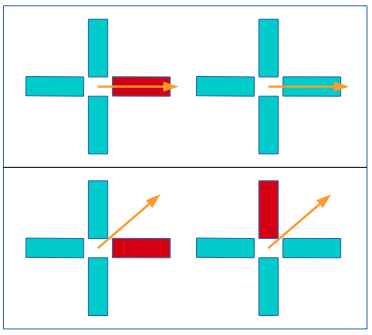
\includegraphics[width=0.5\textwidth]{pulsation.png}
  \caption{Pulsation tacton}
  \label{fig:pulsation}
\end{figure}



\section{Applications}

The HaptiQ can provide a new set of haptic cues which allow the visually impaired to better perceive lines, edges and directions. Two basic applications have been implemented using the API previously described.

\section{NOTES:}

 The HTP provides the following properties through a single point haptic cue \todo[noline]{this paragraph is partially copied from paper} :
\begin{itemize}
\item \textbf{EMPHASIS ON THE DESIGN CHOICES OF HAPTIQ, like not having a break or not doing any texture behaviours}
	\item height and texture: "the relief and tactile feel that corresponds to elements displayed on the table".
    \item malleability: "how different materials respond to touch and pressure".
    \item friction: "resistance to movement in directions parallel to the table plane".
    \item location: "different positions on the table should provide appropriate haptic feedback".
    \item multiplicity: "the ability to provide multi-user or multi-point haptic feedback simultaneously". \cite{marquardt2009haptic}
\end{itemize}


\begin{enumerate}
	\item Hardware design
    	\begin{enumerate}
        \item FIRST ITERATION
            \item touch screen display SDK should be able to provide raw input
            \item from Brock's : "most blind seem to explore tactile maps with both hands and all 10 fingers"
            \item the computer needs a sound card for enabling text-to-speech output
        \end{enumerate}
	\item MHTP API architecture
    	\begin{enumerate}

        	\item Factory pattern with reflection in combination with delegation pattern was used to abstract the input from the touch screen device and notify the MHTP manager system
            \item Observer pattern is used to notify haptic shapes about any new input
            \item Limitations: there is a lower bound threshold on how often input can be acquired. this depends on the input device, the input technique used and the "refresh rate" of the MHTP
            \item texture recognition not impemented because servos cannot act over a certain frequency. Papert \cite{brown2005first} has a part where it says what's the skin frequency range. Solutions could include electro-vibration or haptic vibration motors (http://www.precisionmicrodrives.com/vibrating-vibrator-vibration-motors)
        \end{enumerate}

    \item Text exploration using SpeechSynthetiser - this can be personalised by adding custom haptic shapes which can react differently
\end{enumerate}


